\documentclass[1p]{elsarticle_modified}
%\bibliographystyle{elsarticle-num}

%\usepackage[colorlinks]{hyperref}
%\usepackage{abbrmath_seonhwa} %\Abb, \Ascr, \Acal ,\Abf, \Afrak
\usepackage{amsfonts}
\usepackage{amssymb}
\usepackage{amsmath}
\usepackage{amsthm}
\usepackage{scalefnt}
\usepackage{amsbsy}
\usepackage{kotex}
\usepackage{caption}
\usepackage{subfig}
\usepackage{color}
\usepackage{graphicx}
\usepackage{xcolor} %% white, black, red, green, blue, cyan, magenta, yellow
\usepackage{float}
\usepackage{setspace}
\usepackage{hyperref}

\usepackage{tikz}
\usetikzlibrary{arrows}

\usepackage{multirow}
\usepackage{array} % fixed length table
\usepackage{hhline}

%%%%%%%%%%%%%%%%%%%%%
\makeatletter
\renewcommand*\env@matrix[1][\arraystretch]{%
	\edef\arraystretch{#1}%
	\hskip -\arraycolsep
	\let\@ifnextchar\new@ifnextchar
	\array{*\c@MaxMatrixCols c}}
\makeatother %https://tex.stackexchange.com/questions/14071/how-can-i-increase-the-line-spacing-in-a-matrix
%%%%%%%%%%%%%%%

\usepackage[normalem]{ulem}

\newcommand{\msout}[1]{\ifmmode\text{\sout{\ensuremath{#1}}}\else\sout{#1}\fi}
%SOURCE: \msout is \stkout macro in https://tex.stackexchange.com/questions/20609/strikeout-in-math-mode

\newcommand{\cancel}[1]{
	\ifmmode
	{\color{red}\msout{#1}}
	\else
	{\color{red}\sout{#1}}
	\fi
}

\newcommand{\add}[1]{
	{\color{blue}\uwave{#1}}
}

\newcommand{\replace}[2]{
	\ifmmode
	{\color{red}\msout{#1}}{\color{blue}\uwave{#2}}
	\else
	{\color{red}\sout{#1}}{\color{blue}\uwave{#2}}
	\fi
}

\newcommand{\Sol}{\mathcal{S}} %segment
\newcommand{\D}{D} %diagram
\newcommand{\A}{\mathcal{A}} %arc


%%%%%%%%%%%%%%%%%%%%%%%%%%%%%5 test

\def\sl{\operatorname{\textup{SL}}(2,\Cbb)}
\def\psl{\operatorname{\textup{PSL}}(2,\Cbb)}
\def\quan{\mkern 1mu \triangleright \mkern 1mu}

\theoremstyle{definition}
\newtheorem{thm}{Theorem}[section]
\newtheorem{prop}[thm]{Proposition}
\newtheorem{lem}[thm]{Lemma}
\newtheorem{ques}[thm]{Question}
\newtheorem{cor}[thm]{Corollary}
\newtheorem{defn}[thm]{Definition}
\newtheorem{exam}[thm]{Example}
\newtheorem{rmk}[thm]{Remark}
\newtheorem{alg}[thm]{Algorithm}

\newcommand{\I}{\sqrt{-1}}
\begin{document}

%\begin{frontmatter}
%
%\title{Boundary parabolic representations of knots up to 8 crossings}
%
%%% Group authors per affiliation:
%\author{Yunhi Cho} 
%\address{Department of Mathematics, University of Seoul, Seoul, Korea}
%\ead{yhcho@uos.ac.kr}
%
%
%\author{Seonhwa Kim} %\fnref{s_kim}}
%\address{Center for Geometry and Physics, Institute for Basic Science, Pohang, 37673, Korea}
%\ead{ryeona17@ibs.re.kr}
%
%\author{Hyuk Kim}
%\address{Department of Mathematical Sciences, Seoul National University, Seoul 08826, Korea}
%\ead{hyukkim@snu.ac.kr}
%
%\author{Seokbeom Yoon}
%\address{Department of Mathematical Sciences, Seoul National University, Seoul, 08826,  Korea}
%\ead{sbyoon15@snu.ac.kr}
%
%\begin{abstract}
%We find all boundary parabolic representation of knots up to 8 crossings.
%
%\end{abstract}
%\begin{keyword}
%    \MSC[2010] 57M25 
%\end{keyword}
%
%\end{frontmatter}

%\linenumbers
%\tableofcontents
%
\newcommand\colored[1]{\textcolor{white}{\rule[-0.35ex]{0.8em}{1.4ex}}\kern-0.8em\color{red} #1}%
%\newcommand\colored[1]{\textcolor{white}{ #1}\kern-2.17ex	\textcolor{white}{ #1}\kern-1.81ex	\textcolor{white}{ #1}\kern-2.15ex\color{red}#1	}

{\Large $\underline{12a_{0820}~(K12a_{0820})}$}

\setlength{\tabcolsep}{10pt}
\renewcommand{\arraystretch}{1.6}
\vspace{1cm}\begin{tabular}{m{100pt}>{\centering\arraybackslash}m{274pt}}
\multirow{5}{120pt}{
	\centering
	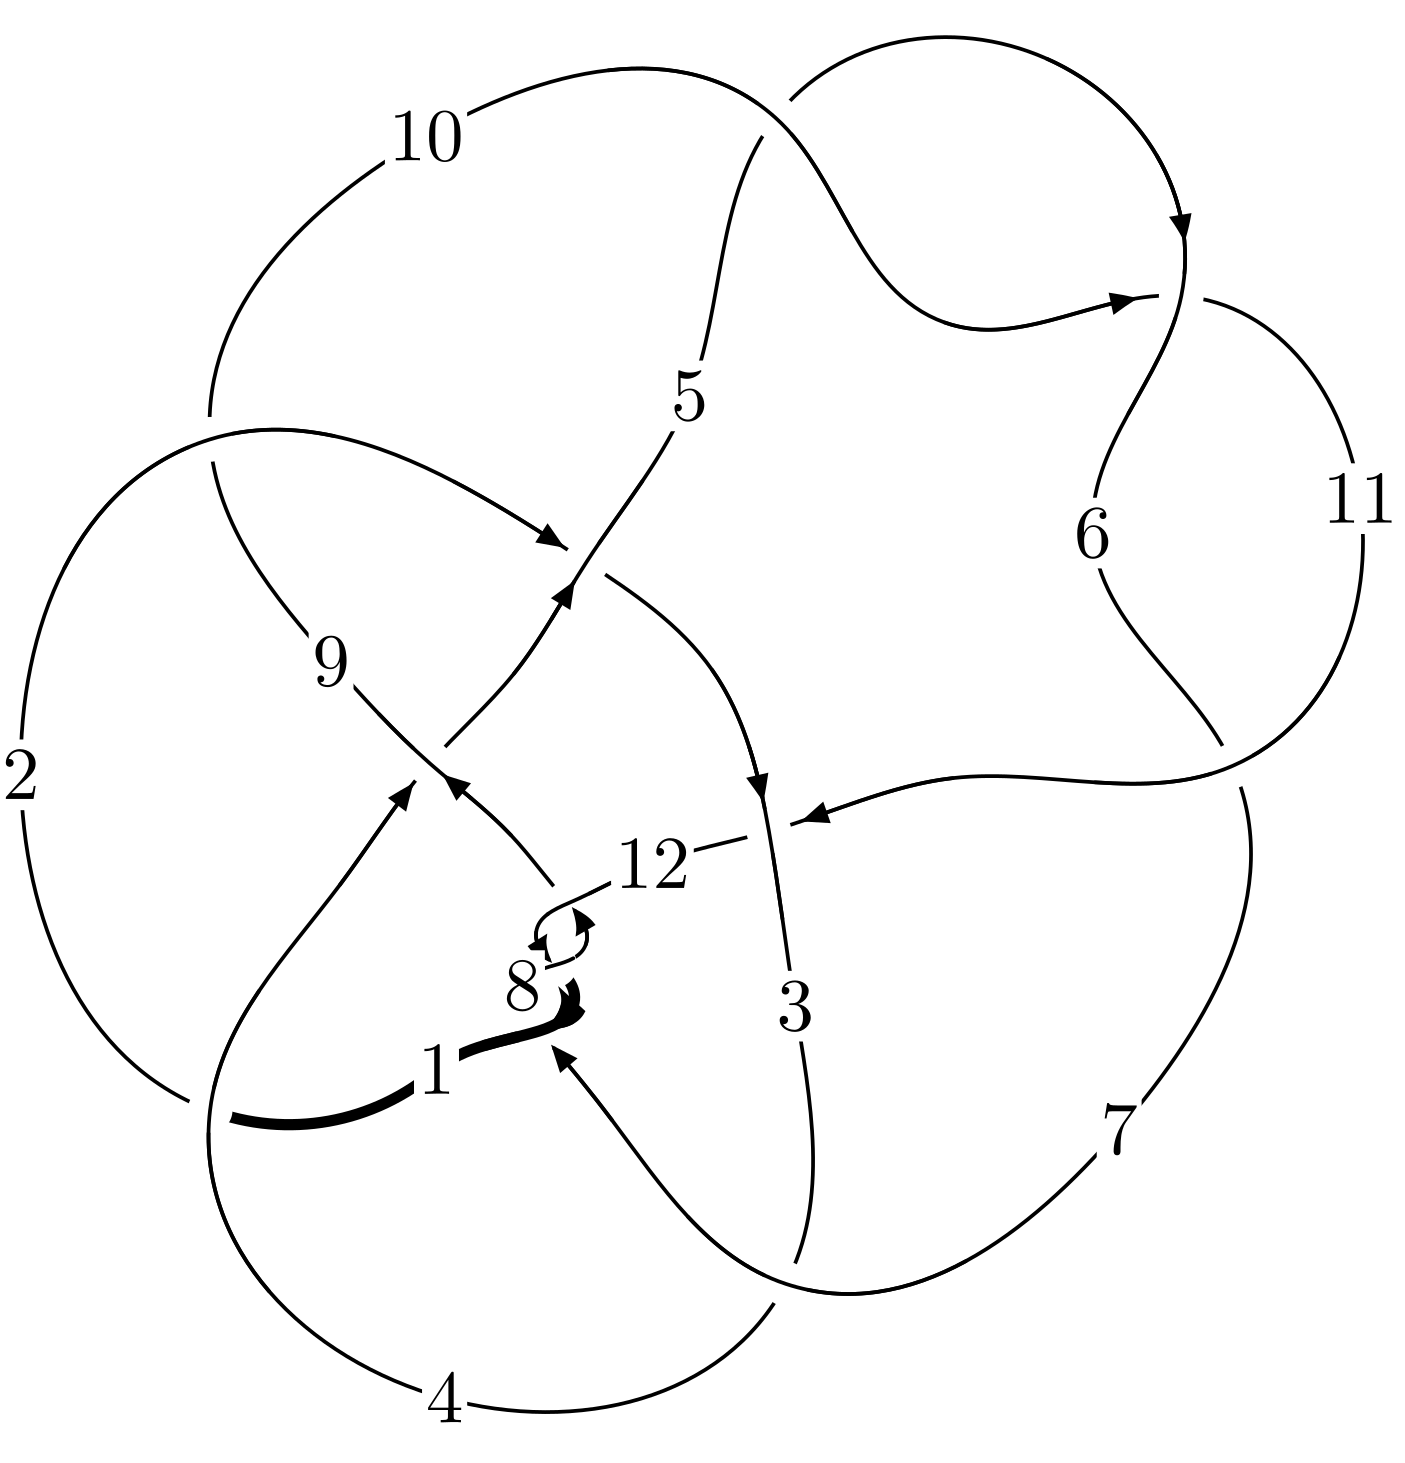
\includegraphics[width=112pt]{../../../GIT/diagram.site/Diagrams/png/1621_12a_0820.png}\\
\ \ \ A knot diagram\footnotemark}&
\allowdisplaybreaks
\textbf{Linearized knot diagam} \\
\cline{2-2}
 &
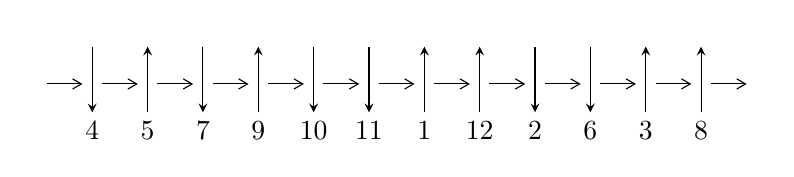
\begin{tikzpicture}[x=20pt, y=17pt]
	% nodes
	\node (C0) at (0, 0) {};
	\node (C1) at (1, 0) {};
	\node (C1U) at (1, +1) {};
	\node (C1D) at (1, -1) {4};

	\node (C2) at (2, 0) {};
	\node (C2U) at (2, +1) {};
	\node (C2D) at (2, -1) {5};

	\node (C3) at (3, 0) {};
	\node (C3U) at (3, +1) {};
	\node (C3D) at (3, -1) {7};

	\node (C4) at (4, 0) {};
	\node (C4U) at (4, +1) {};
	\node (C4D) at (4, -1) {9};

	\node (C5) at (5, 0) {};
	\node (C5U) at (5, +1) {};
	\node (C5D) at (5, -1) {10};

	\node (C6) at (6, 0) {};
	\node (C6U) at (6, +1) {};
	\node (C6D) at (6, -1) {11};

	\node (C7) at (7, 0) {};
	\node (C7U) at (7, +1) {};
	\node (C7D) at (7, -1) {1};

	\node (C8) at (8, 0) {};
	\node (C8U) at (8, +1) {};
	\node (C8D) at (8, -1) {12};

	\node (C9) at (9, 0) {};
	\node (C9U) at (9, +1) {};
	\node (C9D) at (9, -1) {2};

	\node (C10) at (10, 0) {};
	\node (C10U) at (10, +1) {};
	\node (C10D) at (10, -1) {6};

	\node (C11) at (11, 0) {};
	\node (C11U) at (11, +1) {};
	\node (C11D) at (11, -1) {3};

	\node (C12) at (12, 0) {};
	\node (C12U) at (12, +1) {};
	\node (C12D) at (12, -1) {8};
	\node (C13) at (13, 0) {};

	% arrows
	\draw[->,>={angle 60}]
	(C0) edge (C1) (C1) edge (C2) (C2) edge (C3) (C3) edge (C4) (C4) edge (C5) (C5) edge (C6) (C6) edge (C7) (C7) edge (C8) (C8) edge (C9) (C9) edge (C10) (C10) edge (C11) (C11) edge (C12) (C12) edge (C13) ;	\draw[->,>=stealth]
	(C1U) edge (C1D) (C2D) edge (C2U) (C3U) edge (C3D) (C4D) edge (C4U) (C5U) edge (C5D) (C6U) edge (C6D) (C7D) edge (C7U) (C8D) edge (C8U) (C9U) edge (C9D) (C10U) edge (C10D) (C11D) edge (C11U) (C12D) edge (C12U) ;
	\end{tikzpicture} \\
\hhline{~~} \\& 
\textbf{Solving Sequence} \\ \cline{2-2} 
 &
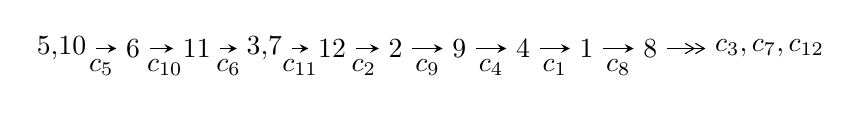
\begin{tikzpicture}[x=23pt, y=7pt]
	% node
	\node (A0) at (-1/8, 0) {5,10};
	\node (A1) at (1, 0) {6};
	\node (A2) at (2, 0) {11};
	\node (A3) at (49/16, 0) {3,7};
	\node (A4) at (33/8, 0) {12};
	\node (A5) at (41/8, 0) {2};
	\node (A6) at (49/8, 0) {9};
	\node (A7) at (57/8, 0) {4};
	\node (A8) at (65/8, 0) {1};
	\node (A9) at (73/8, 0) {8};
	\node (C1) at (1/2, -1) {$c_{5}$};
	\node (C2) at (3/2, -1) {$c_{10}$};
	\node (C3) at (5/2, -1) {$c_{6}$};
	\node (C4) at (29/8, -1) {$c_{11}$};
	\node (C5) at (37/8, -1) {$c_{2}$};
	\node (C6) at (45/8, -1) {$c_{9}$};
	\node (C7) at (53/8, -1) {$c_{4}$};
	\node (C8) at (61/8, -1) {$c_{1}$};
	\node (C9) at (69/8, -1) {$c_{8}$};
	\node (A10) at (11, 0) {$c_{3},c_{7},c_{12}$};

	% edge
	\draw[->,>=stealth]	
	(A0) edge (A1) (A1) edge (A2) (A2) edge (A3) (A3) edge (A4) (A4) edge (A5) (A5) edge (A6) (A6) edge (A7) (A7) edge (A8) (A8) edge (A9) ;
	\draw[->>,>={angle 60}]	
	(A9) edge (A10);
\end{tikzpicture} \\ 

\end{tabular} \\

\footnotetext{
The image of knot diagram is generated by the software ``\textbf{Draw programme}" developed by Andrew Bartholomew(\url{http://www.layer8.co.uk/maths/draw/index.htm\#Running-draw}), where we modified some parts for our purpose(\url{https://github.com/CATsTAILs/LinksPainter}).
}\phantom \\ \newline 
\centering \textbf{Ideals for irreducible components\footnotemark of $X_{\text{par}}$} 
 
\begin{align*}
I^u_{1}&=\langle 
-1.40939\times10^{253} u^{113}-2.02595\times10^{253} u^{112}+\cdots+4.76921\times10^{252} b+1.39224\times10^{253},\\
\phantom{I^u_{1}}&\phantom{= \langle  }-5.54737\times10^{253} u^{113}-8.27027\times10^{253} u^{112}+\cdots+4.76921\times10^{252} a+2.16515\times10^{254},\\
\phantom{I^u_{1}}&\phantom{= \langle  }u^{114}+u^{113}+\cdots-17 u+1\rangle \\
I^u_{2}&=\langle 
1390 u^{24}-1230 u^{23}+\cdots+3407 b-2014,\;97 u^{24}-2733 u^{23}+\cdots+3407 a+6095,\\
\phantom{I^u_{2}}&\phantom{= \langle  }u^{25}-14 u^{23}+\cdots-2 u-1\rangle \\
\\
\end{align*}
\raggedright * 2 irreducible components of $\dim_{\mathbb{C}}=0$, with total 139 representations.\\
\footnotetext{All coefficients of polynomials are rational numbers. But the coefficients are sometimes approximated in decimal forms when there is not enough margin.}
\newpage
\renewcommand{\arraystretch}{1}
\centering \section*{I. $I^u_{1}= \langle -1.41\times10^{253} u^{113}-2.03\times10^{253} u^{112}+\cdots+4.77\times10^{252} b+1.39\times10^{253},\;-5.55\times10^{253} u^{113}-8.27\times10^{253} u^{112}+\cdots+4.77\times10^{252} a+2.17\times10^{254},\;u^{114}+u^{113}+\cdots-17 u+1 \rangle$}
\flushleft \textbf{(i) Arc colorings}\\
\begin{tabular}{m{7pt} m{180pt} m{7pt} m{180pt} }
\flushright $a_{5}=$&$\begin{pmatrix}1\\0\end{pmatrix}$ \\
\flushright $a_{10}=$&$\begin{pmatrix}0\\u\end{pmatrix}$ \\
\flushright $a_{6}=$&$\begin{pmatrix}1\\u^2\end{pmatrix}$ \\
\flushright $a_{11}=$&$\begin{pmatrix}- u\\- u^3+u\end{pmatrix}$ \\
\flushright $a_{3}=$&$\begin{pmatrix}11.6316 u^{113}+17.3410 u^{112}+\cdots+401.267 u-45.3985\\2.95519 u^{113}+4.24799 u^{112}+\cdots+59.4230 u-2.91923\end{pmatrix}$ \\
\flushright $a_{7}=$&$\begin{pmatrix}- u^2+1\\- u^4+2 u^2\end{pmatrix}$ \\
\flushright $a_{12}=$&$\begin{pmatrix}-27.6647 u^{113}-41.0174 u^{112}+\cdots-972.586 u+85.2806\\-4.76338 u^{113}-5.86579 u^{112}+\cdots-156.987 u+9.92136\end{pmatrix}$ \\
\flushright $a_{2}=$&$\begin{pmatrix}8.67645 u^{113}+13.0930 u^{112}+\cdots+341.844 u-42.4792\\2.95519 u^{113}+4.24799 u^{112}+\cdots+59.4230 u-2.91923\end{pmatrix}$ \\
\flushright $a_{9}=$&$\begin{pmatrix}-21.0401 u^{113}-28.9104 u^{112}+\cdots-655.353 u+67.2492\\-4.35621 u^{113}-6.54646 u^{112}+\cdots-150.939 u+9.08524\end{pmatrix}$ \\
\flushright $a_{4}=$&$\begin{pmatrix}13.1028 u^{113}+20.6472 u^{112}+\cdots+487.758 u-52.3250\\3.40344 u^{113}+5.57151 u^{112}+\cdots+89.2902 u-4.94819\end{pmatrix}$ \\
\flushright $a_{1}=$&$\begin{pmatrix}-24.3708 u^{113}-38.2365 u^{112}+\cdots-776.120 u+38.6407\\-6.35400 u^{113}-9.86861 u^{112}+\cdots-249.572 u+17.7461\end{pmatrix}$ \\
\flushright $a_{8}=$&$\begin{pmatrix}7.70870 u^{113}+8.88631 u^{112}+\cdots+180.088 u-2.90069\\3.10824 u^{113}+3.34002 u^{112}+\cdots+77.4664 u-6.10232\end{pmatrix}$\\&\end{tabular}
\flushleft \textbf{(ii) Obstruction class $= -1$}\\~\\
\flushleft \textbf{(iii) Cusp Shapes $= -31.5841 u^{113}-47.8132 u^{112}+\cdots-1054.21 u+82.8491$}\\~\\
\newpage\renewcommand{\arraystretch}{1}
\flushleft \textbf{(iv) u-Polynomials at the component}\newline \\
\begin{tabular}{m{50pt}|m{274pt}}
Crossings & \hspace{64pt}u-Polynomials at each crossing \\
\hline $$\begin{aligned}c_{1}\end{aligned}$$&$\begin{aligned}
&u^{114}+9 u^{113}+\cdots-1176 u+10199
\end{aligned}$\\
\hline $$\begin{aligned}c_{2}\end{aligned}$$&$\begin{aligned}
&u^{114}+13 u^{112}+\cdots+23139 u+2413
\end{aligned}$\\
\hline $$\begin{aligned}c_{3}\end{aligned}$$&$\begin{aligned}
&u^{114}+u^{113}+\cdots-4818480 u+4468393
\end{aligned}$\\
\hline $$\begin{aligned}c_{4}\end{aligned}$$&$\begin{aligned}
&u^{114}-4 u^{112}+\cdots+3 u-1
\end{aligned}$\\
\hline $$\begin{aligned}c_{5},c_{6},c_{10}\end{aligned}$$&$\begin{aligned}
&u^{114}- u^{113}+\cdots+17 u+1
\end{aligned}$\\
\hline $$\begin{aligned}c_{7},c_{8},c_{12}\end{aligned}$$&$\begin{aligned}
&u^{114}+56 u^{112}+\cdots-19 u+1
\end{aligned}$\\
\hline $$\begin{aligned}c_{9}\end{aligned}$$&$\begin{aligned}
&u^{114}- u^{113}+\cdots-38970 u+6329
\end{aligned}$\\
\hline $$\begin{aligned}c_{11}\end{aligned}$$&$\begin{aligned}
&u^{114}+20 u^{112}+\cdots-4121492 u-493777
\end{aligned}$\\
\hline
\end{tabular}\\~\\
\newpage\renewcommand{\arraystretch}{1}
\flushleft \textbf{(v) Riley Polynomials at the component}\newline \\
\begin{tabular}{m{50pt}|m{274pt}}
Crossings & \hspace{64pt}Riley Polynomials at each crossing \\
\hline $$\begin{aligned}c_{1}\end{aligned}$$&$\begin{aligned}
&y^{114}-41 y^{113}+\cdots-15341392906 y+104019601
\end{aligned}$\\
\hline $$\begin{aligned}c_{2}\end{aligned}$$&$\begin{aligned}
&y^{114}+26 y^{113}+\cdots+99866841 y+5822569
\end{aligned}$\\
\hline $$\begin{aligned}c_{3}\end{aligned}$$&$\begin{aligned}
&y^{114}-55 y^{113}+\cdots-760130663350652 y+19966536002449
\end{aligned}$\\
\hline $$\begin{aligned}c_{4}\end{aligned}$$&$\begin{aligned}
&y^{114}-8 y^{113}+\cdots-193 y+1
\end{aligned}$\\
\hline $$\begin{aligned}c_{5},c_{6},c_{10}\end{aligned}$$&$\begin{aligned}
&y^{114}-121 y^{113}+\cdots-237 y+1
\end{aligned}$\\
\hline $$\begin{aligned}c_{7},c_{8},c_{12}\end{aligned}$$&$\begin{aligned}
&y^{114}+112 y^{113}+\cdots-139 y+1
\end{aligned}$\\
\hline $$\begin{aligned}c_{9}\end{aligned}$$&$\begin{aligned}
&y^{114}-37 y^{113}+\cdots-2516693568 y+40056241
\end{aligned}$\\
\hline $$\begin{aligned}c_{11}\end{aligned}$$&$\begin{aligned}
&y^{114}+40 y^{113}+\cdots+9893819447934 y+243815725729
\end{aligned}$\\
\hline
\end{tabular}\\~\\
\newpage\flushleft \textbf{(vi) Complex Volumes and Cusp Shapes}
$$\begin{array}{c|c|c}  
\text{Solutions to }I^u_{1}& \I (\text{vol} + \sqrt{-1}CS) & \text{Cusp shape}\\
 \hline 
\begin{aligned}
u &= -0.504390 + 0.859932 I \\
a &= -0.318445 + 0.156899 I \\
b &= -0.019841 + 1.001800 I\end{aligned}
 & -9.00028 + 4.07227 I & \phantom{-0.000000 } 0 \\ \hline\begin{aligned}
u &= -0.504390 - 0.859932 I \\
a &= -0.318445 - 0.156899 I \\
b &= -0.019841 - 1.001800 I\end{aligned}
 & -9.00028 - 4.07227 I & \phantom{-0.000000 } 0 \\ \hline\begin{aligned}
u &= \phantom{-}0.627792 + 0.808125 I \\
a &= \phantom{-}0.504608 + 0.487111 I \\
b &= -0.735286 + 0.803959 I\end{aligned}
 & -1.68248 - 4.28082 I & \phantom{-0.000000 } 0 \\ \hline\begin{aligned}
u &= \phantom{-}0.627792 - 0.808125 I \\
a &= \phantom{-}0.504608 - 0.487111 I \\
b &= -0.735286 - 0.803959 I\end{aligned}
 & -1.68248 + 4.28082 I & \phantom{-0.000000 } 0 \\ \hline\begin{aligned}
u &= -0.624670 + 0.747433 I \\
a &= \phantom{-}0.745136 - 0.536061 I \\
b &= -0.459020 - 0.938010 I\end{aligned}
 & -9.48244 + 1.28540 I & \phantom{-0.000000 } 0 \\ \hline\begin{aligned}
u &= -0.624670 - 0.747433 I \\
a &= \phantom{-}0.745136 + 0.536061 I \\
b &= -0.459020 + 0.938010 I\end{aligned}
 & -9.48244 - 1.28540 I & \phantom{-0.000000 } 0 \\ \hline\begin{aligned}
u &= \phantom{-}0.648355 + 0.795879 I \\
a &= \phantom{-}0.385231 + 0.691676 I \\
b &= -0.951220 + 1.028110 I\end{aligned}
 & -7.2766 - 13.7621 I & \phantom{-0.000000 } 0 \\ \hline\begin{aligned}
u &= \phantom{-}0.648355 - 0.795879 I \\
a &= \phantom{-}0.385231 - 0.691676 I \\
b &= -0.951220 - 1.028110 I\end{aligned}
 & -7.2766 + 13.7621 I & \phantom{-0.000000 } 0 \\ \hline\begin{aligned}
u &= -0.648247 + 0.798822 I \\
a &= \phantom{-}0.407999 - 0.595360 I \\
b &= -0.894448 - 0.909448 I\end{aligned}
 & -0.89385 + 9.60187 I & \phantom{-0.000000 } 0 \\ \hline\begin{aligned}
u &= -0.648247 - 0.798822 I \\
a &= \phantom{-}0.407999 + 0.595360 I \\
b &= -0.894448 + 0.909448 I\end{aligned}
 & -0.89385 - 9.60187 I & \phantom{-0.000000 } 0\\
 \hline 
 \end{array}$$\newpage$$\begin{array}{c|c|c}  
\text{Solutions to }I^u_{1}& \I (\text{vol} + \sqrt{-1}CS) & \text{Cusp shape}\\
 \hline 
\begin{aligned}
u &= \phantom{-}0.469837 + 0.938728 I \\
a &= -0.404972 + 0.279102 I \\
b &= -0.567103 - 0.722810 I\end{aligned}
 & -6.66315 + 8.11811 I & \phantom{-0.000000 } 0 \\ \hline\begin{aligned}
u &= \phantom{-}0.469837 - 0.938728 I \\
a &= -0.404972 - 0.279102 I \\
b &= -0.567103 + 0.722810 I\end{aligned}
 & -6.66315 - 8.11811 I & \phantom{-0.000000 } 0 \\ \hline\begin{aligned}
u &= -1.023880 + 0.242312 I \\
a &= \phantom{-}1.41856 + 0.48183 I \\
b &= \phantom{-}0.790054 - 0.125048 I\end{aligned}
 & -5.01066 + 0.32843 I & \phantom{-0.000000 } 0 \\ \hline\begin{aligned}
u &= -1.023880 - 0.242312 I \\
a &= \phantom{-}1.41856 - 0.48183 I \\
b &= \phantom{-}0.790054 + 0.125048 I\end{aligned}
 & -5.01066 - 0.32843 I & \phantom{-0.000000 } 0 \\ \hline\begin{aligned}
u &= -0.840937 + 0.428235 I \\
a &= \phantom{-}1.45683 - 0.06660 I \\
b &= \phantom{-}0.576258 - 0.637825 I\end{aligned}
 & -5.65724 - 0.96064 I & \phantom{-0.000000 } 0 \\ \hline\begin{aligned}
u &= -0.840937 - 0.428235 I \\
a &= \phantom{-}1.45683 + 0.06660 I \\
b &= \phantom{-}0.576258 + 0.637825 I\end{aligned}
 & -5.65724 + 0.96064 I & \phantom{-0.000000 } 0 \\ \hline\begin{aligned}
u &= \phantom{-}0.684025 + 0.608244 I \\
a &= \phantom{-}0.108560 - 0.218368 I \\
b &= \phantom{-}0.374450 - 0.458339 I\end{aligned}
 & -1.22956 - 1.97374 I & \phantom{-0.000000 } 0 \\ \hline\begin{aligned}
u &= \phantom{-}0.684025 - 0.608244 I \\
a &= \phantom{-}0.108560 + 0.218368 I \\
b &= \phantom{-}0.374450 + 0.458339 I\end{aligned}
 & -1.22956 + 1.97374 I & \phantom{-0.000000 } 0 \\ \hline\begin{aligned}
u &= -0.480454 + 0.988671 I \\
a &= -0.237939 - 0.221262 I \\
b &= -0.424825 + 0.602509 I\end{aligned}
 & -0.26142 - 3.85934 I & \phantom{-0.000000 } 0 \\ \hline\begin{aligned}
u &= -0.480454 - 0.988671 I \\
a &= -0.237939 + 0.221262 I \\
b &= -0.424825 - 0.602509 I\end{aligned}
 & -0.26142 + 3.85934 I & \phantom{-0.000000 } 0\\
 \hline 
 \end{array}$$\newpage$$\begin{array}{c|c|c}  
\text{Solutions to }I^u_{1}& \I (\text{vol} + \sqrt{-1}CS) & \text{Cusp shape}\\
 \hline 
\begin{aligned}
u &= \phantom{-}0.847240 + 0.275289 I \\
a &= \phantom{-}1.307420 - 0.150491 I \\
b &= \phantom{-}0.546342 + 0.345590 I\end{aligned}
 & -0.653113 + 0.203450 I & \phantom{-0.000000 } 0 \\ \hline\begin{aligned}
u &= \phantom{-}0.847240 - 0.275289 I \\
a &= \phantom{-}1.307420 + 0.150491 I \\
b &= \phantom{-}0.546342 - 0.345590 I\end{aligned}
 & -0.653113 - 0.203450 I & \phantom{-0.000000 } 0 \\ \hline\begin{aligned}
u &= \phantom{-}1.12255\phantom{ +0.000000I} \\
a &= \phantom{-}0.954007\phantom{ +0.000000I} \\
b &= -0.662366\phantom{ +0.000000I}\end{aligned}
 & -1.71869\phantom{ +0.000000I} & \phantom{-0.000000 } 0 \\ \hline\begin{aligned}
u &= \phantom{-}0.637119 + 0.961400 I \\
a &= -0.140987 + 0.024677 I \\
b &= -0.116157 - 0.576022 I\end{aligned}
 & -1.37866 - 1.56456 I & \phantom{-0.000000 } 0 \\ \hline\begin{aligned}
u &= \phantom{-}0.637119 - 0.961400 I \\
a &= -0.140987 - 0.024677 I \\
b &= -0.116157 + 0.576022 I\end{aligned}
 & -1.37866 + 1.56456 I & \phantom{-0.000000 } 0 \\ \hline\begin{aligned}
u &= -0.268034 + 0.682036 I \\
a &= -0.243151 + 0.202685 I \\
b &= \phantom{-}0.83284 + 1.16863 I\end{aligned}
 & -3.87371 + 4.99652 I & \phantom{-0.000000 } 0 \\ \hline\begin{aligned}
u &= -0.268034 - 0.682036 I \\
a &= -0.243151 - 0.202685 I \\
b &= \phantom{-}0.83284 - 1.16863 I\end{aligned}
 & -3.87371 - 4.99652 I & \phantom{-0.000000 } 0 \\ \hline\begin{aligned}
u &= \phantom{-}0.215671 + 0.695262 I \\
a &= \phantom{-}0.802229 - 0.072153 I \\
b &= -0.362588 + 0.284379 I\end{aligned}
 & -0.01282 - 1.97773 I & \phantom{-0.000000 } 0 \\ \hline\begin{aligned}
u &= \phantom{-}0.215671 - 0.695262 I \\
a &= \phantom{-}0.802229 + 0.072153 I \\
b &= -0.362588 - 0.284379 I\end{aligned}
 & -0.01282 + 1.97773 I & \phantom{-0.000000 } 0 \\ \hline\begin{aligned}
u &= \phantom{-}0.492943 + 0.502644 I \\
a &= \phantom{-}0.344711 - 0.916714 I \\
b &= \phantom{-}1.051700 - 0.405957 I\end{aligned}
 & -1.76151 - 1.77369 I & \phantom{-0.000000 } 0\\
 \hline 
 \end{array}$$\newpage$$\begin{array}{c|c|c}  
\text{Solutions to }I^u_{1}& \I (\text{vol} + \sqrt{-1}CS) & \text{Cusp shape}\\
 \hline 
\begin{aligned}
u &= \phantom{-}0.492943 - 0.502644 I \\
a &= \phantom{-}0.344711 + 0.916714 I \\
b &= \phantom{-}1.051700 + 0.405957 I\end{aligned}
 & -1.76151 + 1.77369 I & \phantom{-0.000000 } 0 \\ \hline\begin{aligned}
u &= -0.606585 + 0.331100 I \\
a &= \phantom{-}0.257474 + 0.237231 I \\
b &= -1.212140 + 0.308455 I\end{aligned}
 & -6.71204 - 3.43393 I & \phantom{-0.000000 } 0 \\ \hline\begin{aligned}
u &= -0.606585 - 0.331100 I \\
a &= \phantom{-}0.257474 - 0.237231 I \\
b &= -1.212140 - 0.308455 I\end{aligned}
 & -6.71204 + 3.43393 I & \phantom{-0.000000 } 0 \\ \hline\begin{aligned}
u &= \phantom{-}0.544241 + 0.423178 I \\
a &= -0.52745 - 1.60285 I \\
b &= \phantom{-}0.97691 - 1.08962 I\end{aligned}
 & -3.11521 - 4.90569 I & \phantom{-0.000000 } 0 \\ \hline\begin{aligned}
u &= \phantom{-}0.544241 - 0.423178 I \\
a &= -0.52745 + 1.60285 I \\
b &= \phantom{-}0.97691 + 1.08962 I\end{aligned}
 & -3.11521 + 4.90569 I & \phantom{-0.000000 } 0 \\ \hline\begin{aligned}
u &= -0.483700 + 0.484947 I \\
a &= -0.344554 + 1.058150 I \\
b &= \phantom{-}0.934790 + 0.863090 I\end{aligned}
 & \phantom{-}1.47204 + 3.21737 I & \phantom{-0.000000 } 0 \\ \hline\begin{aligned}
u &= -0.483700 - 0.484947 I \\
a &= -0.344554 - 1.058150 I \\
b &= \phantom{-}0.934790 - 0.863090 I\end{aligned}
 & \phantom{-}1.47204 - 3.21737 I & \phantom{-0.000000 } 0 \\ \hline\begin{aligned}
u &= \phantom{-}0.641724 + 0.077644 I \\
a &= \phantom{-}0.749700 - 0.145346 I \\
b &= -0.578203 - 0.240264 I\end{aligned}
 & -1.43760 - 0.04845 I & -6.99647 + 0. I\phantom{ +0.000000I} \\ \hline\begin{aligned}
u &= \phantom{-}0.641724 - 0.077644 I \\
a &= \phantom{-}0.749700 + 0.145346 I \\
b &= -0.578203 + 0.240264 I\end{aligned}
 & -1.43760 + 0.04845 I & -6.99647 + 0. I\phantom{ +0.000000I} \\ \hline\begin{aligned}
u &= \phantom{-}1.354950 + 0.073307 I \\
a &= \phantom{-}0.502957 + 1.294070 I \\
b &= \phantom{-}0.001361 + 0.562562 I\end{aligned}
 & -3.08633 - 0.14371 I & \phantom{-0.000000 } 0\\
 \hline 
 \end{array}$$\newpage$$\begin{array}{c|c|c}  
\text{Solutions to }I^u_{1}& \I (\text{vol} + \sqrt{-1}CS) & \text{Cusp shape}\\
 \hline 
\begin{aligned}
u &= \phantom{-}1.354950 - 0.073307 I \\
a &= \phantom{-}0.502957 - 1.294070 I \\
b &= \phantom{-}0.001361 - 0.562562 I\end{aligned}
 & -3.08633 + 0.14371 I & \phantom{-0.000000 } 0 \\ \hline\begin{aligned}
u &= -1.356960 + 0.261061 I \\
a &= \phantom{-}0.535902 - 0.852694 I \\
b &= -0.694855 - 0.462533 I\end{aligned}
 & -4.99408 + 5.47655 I & \phantom{-0.000000 } 0 \\ \hline\begin{aligned}
u &= -1.356960 - 0.261061 I \\
a &= \phantom{-}0.535902 + 0.852694 I \\
b &= -0.694855 + 0.462533 I\end{aligned}
 & -4.99408 - 5.47655 I & \phantom{-0.000000 } 0 \\ \hline\begin{aligned}
u &= \phantom{-}0.264417 + 0.558492 I \\
a &= -0.528334 - 0.121740 I \\
b &= \phantom{-}0.879406 - 0.976250 I\end{aligned}
 & \phantom{-}1.10020 - 3.44919 I & \phantom{-}7.33497 + 9.15225 I \\ \hline\begin{aligned}
u &= \phantom{-}0.264417 - 0.558492 I \\
a &= -0.528334 + 0.121740 I \\
b &= \phantom{-}0.879406 + 0.976250 I\end{aligned}
 & \phantom{-}1.10020 + 3.44919 I & \phantom{-}7.33497 - 9.15225 I \\ \hline\begin{aligned}
u &= -1.401100 + 0.022072 I \\
a &= \phantom{-}0.60160 + 1.55230 I \\
b &= \phantom{-}0.159019 + 1.035610 I\end{aligned}
 & -8.01156 + 2.83142 I & \phantom{-0.000000 } 0 \\ \hline\begin{aligned}
u &= -1.401100 - 0.022072 I \\
a &= \phantom{-}0.60160 - 1.55230 I \\
b &= \phantom{-}0.159019 - 1.035610 I\end{aligned}
 & -8.01156 - 2.83142 I & \phantom{-0.000000 } 0 \\ \hline\begin{aligned}
u &= -1.402530 + 0.127614 I \\
a &= \phantom{-}0.15023 - 1.68921 I \\
b &= -0.165522 - 0.371500 I\end{aligned}
 & -4.20035 + 4.68431 I & \phantom{-0.000000 } 0 \\ \hline\begin{aligned}
u &= -1.402530 - 0.127614 I \\
a &= \phantom{-}0.15023 + 1.68921 I \\
b &= -0.165522 + 0.371500 I\end{aligned}
 & -4.20035 - 4.68431 I & \phantom{-0.000000 } 0 \\ \hline\begin{aligned}
u &= -0.312958 + 0.484410 I \\
a &= \phantom{-}0.68470 - 2.52421 I \\
b &= -0.647033 - 0.214427 I\end{aligned}
 & -5.73034 + 6.37831 I & -0.93847 - 10.47810 I\\
 \hline 
 \end{array}$$\newpage$$\begin{array}{c|c|c}  
\text{Solutions to }I^u_{1}& \I (\text{vol} + \sqrt{-1}CS) & \text{Cusp shape}\\
 \hline 
\begin{aligned}
u &= -0.312958 - 0.484410 I \\
a &= \phantom{-}0.68470 + 2.52421 I \\
b &= -0.647033 + 0.214427 I\end{aligned}
 & -5.73034 - 6.37831 I & -0.93847 + 10.47810 I \\ \hline\begin{aligned}
u &= \phantom{-}1.42402 + 0.19507 I \\
a &= \phantom{-}0.18091 - 2.16307 I \\
b &= \phantom{-}0.95293 - 1.81419 I\end{aligned}
 & -9.28920 - 8.06698 I & \phantom{-0.000000 } 0 \\ \hline\begin{aligned}
u &= \phantom{-}1.42402 - 0.19507 I \\
a &= \phantom{-}0.18091 + 2.16307 I \\
b &= \phantom{-}0.95293 + 1.81419 I\end{aligned}
 & -9.28920 + 8.06698 I & \phantom{-0.000000 } 0 \\ \hline\begin{aligned}
u &= \phantom{-}1.43696 + 0.07142 I \\
a &= \phantom{-}0.50611 - 1.59958 I \\
b &= \phantom{-}1.41616 - 1.19115 I\end{aligned}
 & -7.09296 - 3.71047 I & \phantom{-0.000000 } 0 \\ \hline\begin{aligned}
u &= \phantom{-}1.43696 - 0.07142 I \\
a &= \phantom{-}0.50611 + 1.59958 I \\
b &= \phantom{-}1.41616 + 1.19115 I\end{aligned}
 & -7.09296 + 3.71047 I & \phantom{-0.000000 } 0 \\ \hline\begin{aligned}
u &= \phantom{-}0.149924 + 0.540211 I \\
a &= \phantom{-}1.52053 + 1.40815 I \\
b &= -0.523492 + 0.034626 I\end{aligned}
 & \phantom{-}0.73545 - 2.45150 I & \phantom{-}7.79919 + 8.48403 I \\ \hline\begin{aligned}
u &= \phantom{-}0.149924 - 0.540211 I \\
a &= \phantom{-}1.52053 - 1.40815 I \\
b &= -0.523492 - 0.034626 I\end{aligned}
 & \phantom{-}0.73545 + 2.45150 I & \phantom{-}7.79919 - 8.48403 I \\ \hline\begin{aligned}
u &= -1.44341\phantom{ +0.000000I} \\
a &= \phantom{-}0.0236738\phantom{ +0.000000I} \\
b &= \phantom{-}1.32265\phantom{ +0.000000I}\end{aligned}
 & -4.28765\phantom{ +0.000000I} & \phantom{-0.000000 } 0 \\ \hline\begin{aligned}
u &= -1.44154 + 0.14492 I \\
a &= \phantom{-}0.35936 + 2.03022 I \\
b &= \phantom{-}1.12170 + 1.62153 I\end{aligned}
 & -4.43773 + 5.84177 I & \phantom{-0.000000 } 0 \\ \hline\begin{aligned}
u &= -1.44154 - 0.14492 I \\
a &= \phantom{-}0.35936 - 2.03022 I \\
b &= \phantom{-}1.12170 - 1.62153 I\end{aligned}
 & -4.43773 - 5.84177 I & \phantom{-0.000000 } 0\\
 \hline 
 \end{array}$$\newpage$$\begin{array}{c|c|c}  
\text{Solutions to }I^u_{1}& \I (\text{vol} + \sqrt{-1}CS) & \text{Cusp shape}\\
 \hline 
\begin{aligned}
u &= \phantom{-}1.45794 + 0.12566 I \\
a &= -0.40239 + 1.93795 I \\
b &= -0.195324 + 0.429208 I\end{aligned}
 & -11.5157 - 8.4504 I & \phantom{-0.000000 } 0 \\ \hline\begin{aligned}
u &= \phantom{-}1.45794 - 0.12566 I \\
a &= -0.40239 - 1.93795 I \\
b &= -0.195324 - 0.429208 I\end{aligned}
 & -11.5157 + 8.4504 I & \phantom{-0.000000 } 0 \\ \hline\begin{aligned}
u &= -0.439200 + 0.298658 I \\
a &= \phantom{-}0.993486 + 0.633929 I \\
b &= \phantom{-}0.780963 - 0.210476 I\end{aligned}
 & \phantom{-}1.51577 - 0.17955 I & \phantom{-}6.48644 - 0.46789 I \\ \hline\begin{aligned}
u &= -0.439200 - 0.298658 I \\
a &= \phantom{-}0.993486 - 0.633929 I \\
b &= \phantom{-}0.780963 + 0.210476 I\end{aligned}
 & \phantom{-}1.51577 + 0.17955 I & \phantom{-}6.48644 + 0.46789 I \\ \hline\begin{aligned}
u &= \phantom{-}1.46868 + 0.04128 I \\
a &= -0.04562 - 1.41394 I \\
b &= \phantom{-}1.057150 - 0.865190 I\end{aligned}
 & -7.16622 - 3.90834 I & \phantom{-0.000000 } 0 \\ \hline\begin{aligned}
u &= \phantom{-}1.46868 - 0.04128 I \\
a &= -0.04562 + 1.41394 I \\
b &= \phantom{-}1.057150 + 0.865190 I\end{aligned}
 & -7.16622 + 3.90834 I & \phantom{-0.000000 } 0 \\ \hline\begin{aligned}
u &= -1.50091 + 0.05304 I \\
a &= -1.17889 + 2.04349 I \\
b &= -1.60569 + 1.96668 I\end{aligned}
 & -13.9951 + 6.9232 I & \phantom{-0.000000 } 0 \\ \hline\begin{aligned}
u &= -1.50091 - 0.05304 I \\
a &= -1.17889 - 2.04349 I \\
b &= -1.60569 - 1.96668 I\end{aligned}
 & -13.9951 - 6.9232 I & \phantom{-0.000000 } 0 \\ \hline\begin{aligned}
u &= \phantom{-}1.50232 + 0.04092 I \\
a &= -0.76440 - 1.75414 I \\
b &= -1.23649 - 1.62891 I\end{aligned}
 & -8.15068 - 3.87708 I & \phantom{-0.000000 } 0 \\ \hline\begin{aligned}
u &= \phantom{-}1.50232 - 0.04092 I \\
a &= -0.76440 + 1.75414 I \\
b &= -1.23649 + 1.62891 I\end{aligned}
 & -8.15068 + 3.87708 I & \phantom{-0.000000 } 0\\
 \hline 
 \end{array}$$\newpage$$\begin{array}{c|c|c}  
\text{Solutions to }I^u_{1}& \I (\text{vol} + \sqrt{-1}CS) & \text{Cusp shape}\\
 \hline 
\begin{aligned}
u &= -1.51959 + 0.02383 I \\
a &= -0.46121 + 1.97396 I \\
b &= \phantom{-}0.553037 + 1.032860 I\end{aligned}
 & -14.7160 + 5.6858 I & \phantom{-0.000000 } 0 \\ \hline\begin{aligned}
u &= -1.51959 - 0.02383 I \\
a &= -0.46121 - 1.97396 I \\
b &= \phantom{-}0.553037 - 1.032860 I\end{aligned}
 & -14.7160 - 5.6858 I & \phantom{-0.000000 } 0 \\ \hline\begin{aligned}
u &= \phantom{-}0.478423 + 0.013444 I \\
a &= -2.02485 - 3.24717 I \\
b &= \phantom{-}0.112636 - 0.976226 I\end{aligned}
 & -7.97267 - 5.43473 I & -12.51083 + 5.12901 I \\ \hline\begin{aligned}
u &= \phantom{-}0.478423 - 0.013444 I \\
a &= -2.02485 + 3.24717 I \\
b &= \phantom{-}0.112636 + 0.976226 I\end{aligned}
 & -7.97267 + 5.43473 I & -12.51083 - 5.12901 I \\ \hline\begin{aligned}
u &= -1.52521 + 0.01741 I \\
a &= -0.506949 + 1.014550 I \\
b &= -1.11422 + 0.89488 I\end{aligned}
 & -8.52935 + 0.38383 I & \phantom{-0.000000 } 0 \\ \hline\begin{aligned}
u &= -1.52521 - 0.01741 I \\
a &= -0.506949 - 1.014550 I \\
b &= -1.11422 - 0.89488 I\end{aligned}
 & -8.52935 - 0.38383 I & \phantom{-0.000000 } 0 \\ \hline\begin{aligned}
u &= \phantom{-}1.52396 + 0.14016 I \\
a &= \phantom{-}0.45909 - 2.03397 I \\
b &= \phantom{-}0.98148 - 1.47676 I\end{aligned}
 & -5.21863 - 5.44789 I & \phantom{-0.000000 } 0 \\ \hline\begin{aligned}
u &= \phantom{-}1.52396 - 0.14016 I \\
a &= \phantom{-}0.45909 + 2.03397 I \\
b &= \phantom{-}0.98148 + 1.47676 I\end{aligned}
 & -5.21863 + 5.44789 I & \phantom{-0.000000 } 0 \\ \hline\begin{aligned}
u &= -0.438957 + 0.119226 I \\
a &= \phantom{-}0.960231 + 0.801247 I \\
b &= -0.524651 + 1.117990 I\end{aligned}
 & -1.65555 + 3.25950 I & -8.15736 - 8.85887 I \\ \hline\begin{aligned}
u &= -0.438957 - 0.119226 I \\
a &= \phantom{-}0.960231 - 0.801247 I \\
b &= -0.524651 - 1.117990 I\end{aligned}
 & -1.65555 - 3.25950 I & -8.15736 + 8.85887 I\\
 \hline 
 \end{array}$$\newpage$$\begin{array}{c|c|c}  
\text{Solutions to }I^u_{1}& \I (\text{vol} + \sqrt{-1}CS) & \text{Cusp shape}\\
 \hline 
\begin{aligned}
u &= -1.54161 + 0.12665 I \\
a &= \phantom{-}0.40347 + 2.26598 I \\
b &= \phantom{-}0.93018 + 1.54252 I\end{aligned}
 & -10.10470 + 6.91096 I & \phantom{-0.000000 } 0 \\ \hline\begin{aligned}
u &= -1.54161 - 0.12665 I \\
a &= \phantom{-}0.40347 - 2.26598 I \\
b &= \phantom{-}0.93018 - 1.54252 I\end{aligned}
 & -10.10470 - 6.91096 I & \phantom{-0.000000 } 0 \\ \hline\begin{aligned}
u &= -1.54474 + 0.14832 I \\
a &= \phantom{-}0.71374 + 1.71782 I \\
b &= \phantom{-}1.06815 + 1.34991 I\end{aligned}
 & -8.65341 + 4.05651 I & \phantom{-0.000000 } 0 \\ \hline\begin{aligned}
u &= -1.54474 - 0.14832 I \\
a &= \phantom{-}0.71374 - 1.71782 I \\
b &= \phantom{-}1.06815 - 1.34991 I\end{aligned}
 & -8.65341 - 4.05651 I & \phantom{-0.000000 } 0 \\ \hline\begin{aligned}
u &= \phantom{-}1.55267 + 0.05487 I \\
a &= -1.28419 - 0.59457 I \\
b &= -1.87290 - 0.60942 I\end{aligned}
 & -13.9907 + 2.2313 I & \phantom{-0.000000 } 0 \\ \hline\begin{aligned}
u &= \phantom{-}1.55267 - 0.05487 I \\
a &= -1.28419 + 0.59457 I \\
b &= -1.87290 + 0.60942 I\end{aligned}
 & -13.9907 - 2.2313 I & \phantom{-0.000000 } 0 \\ \hline\begin{aligned}
u &= -1.56260\phantom{ +0.000000I} \\
a &= \phantom{-}0.0873587\phantom{ +0.000000I} \\
b &= -0.700466\phantom{ +0.000000I}\end{aligned}
 & -8.57207\phantom{ +0.000000I} & \phantom{-0.000000 } 0 \\ \hline\begin{aligned}
u &= -0.041627 + 0.430998 I \\
a &= -0.489627 - 1.060360 I \\
b &= \phantom{-}1.073510 + 0.717562 I\end{aligned}
 & -2.07764 + 2.42432 I & \phantom{-}0.50120 - 1.46569 I \\ \hline\begin{aligned}
u &= -0.041627 - 0.430998 I \\
a &= -0.489627 + 1.060360 I \\
b &= \phantom{-}1.073510 - 0.717562 I\end{aligned}
 & -2.07764 - 2.42432 I & \phantom{-}0.50120 + 1.46569 I \\ \hline\begin{aligned}
u &= \phantom{-}0.388339 + 0.174789 I \\
a &= \phantom{-}0.695122 - 1.172320 I \\
b &= -0.89212 - 1.44065 I\end{aligned}
 & -7.61463 - 6.10438 I & -12.9267 + 9.7942 I\\
 \hline 
 \end{array}$$\newpage$$\begin{array}{c|c|c}  
\text{Solutions to }I^u_{1}& \I (\text{vol} + \sqrt{-1}CS) & \text{Cusp shape}\\
 \hline 
\begin{aligned}
u &= \phantom{-}0.388339 - 0.174789 I \\
a &= \phantom{-}0.695122 + 1.172320 I \\
b &= -0.89212 + 1.44065 I\end{aligned}
 & -7.61463 + 6.10438 I & -12.9267 - 9.7942 I \\ \hline\begin{aligned}
u &= \phantom{-}1.56257 + 0.24563 I \\
a &= \phantom{-}0.21949 + 1.50423 I \\
b &= -0.789212 + 1.115810 I\end{aligned}
 & -16.6601 - 4.9317 I & \phantom{-0.000000 } 0 \\ \hline\begin{aligned}
u &= \phantom{-}1.56257 - 0.24563 I \\
a &= \phantom{-}0.21949 - 1.50423 I \\
b &= -0.789212 - 1.115810 I\end{aligned}
 & -16.6601 + 4.9317 I & \phantom{-0.000000 } 0 \\ \hline\begin{aligned}
u &= \phantom{-}1.58321 + 0.04226 I \\
a &= \phantom{-}0.675518 + 0.554970 I \\
b &= -0.246897 + 0.415423 I\end{aligned}
 & -13.88100 - 0.23649 I & \phantom{-0.000000 } 0 \\ \hline\begin{aligned}
u &= \phantom{-}1.58321 - 0.04226 I \\
a &= \phantom{-}0.675518 - 0.554970 I \\
b &= -0.246897 - 0.415423 I\end{aligned}
 & -13.88100 + 0.23649 I & \phantom{-0.000000 } 0 \\ \hline\begin{aligned}
u &= \phantom{-}1.55592 + 0.30385 I \\
a &= -0.412535 - 1.349550 I \\
b &= \phantom{-}0.255020 - 1.333670 I\end{aligned}
 & -15.7486 - 8.3628 I & \phantom{-0.000000 } 0 \\ \hline\begin{aligned}
u &= \phantom{-}1.55592 - 0.30385 I \\
a &= -0.412535 + 1.349550 I \\
b &= \phantom{-}0.255020 + 1.333670 I\end{aligned}
 & -15.7486 + 8.3628 I & \phantom{-0.000000 } 0 \\ \hline\begin{aligned}
u &= -1.57225 + 0.26757 I \\
a &= -0.06011 - 1.49912 I \\
b &= -1.03443 - 1.12243 I\end{aligned}
 & -8.88839 + 8.23460 I & \phantom{-0.000000 } 0 \\ \hline\begin{aligned}
u &= -1.57225 - 0.26757 I \\
a &= -0.06011 + 1.49912 I \\
b &= -1.03443 + 1.12243 I\end{aligned}
 & -8.88839 - 8.23460 I & \phantom{-0.000000 } 0 \\ \hline\begin{aligned}
u &= \phantom{-}1.58087 + 0.26673 I \\
a &= -0.18210 + 1.65020 I \\
b &= -1.13316 + 1.25352 I\end{aligned}
 & -8.2065 - 13.5471 I & \phantom{-0.000000 } 0\\
 \hline 
 \end{array}$$\newpage$$\begin{array}{c|c|c}  
\text{Solutions to }I^u_{1}& \I (\text{vol} + \sqrt{-1}CS) & \text{Cusp shape}\\
 \hline 
\begin{aligned}
u &= \phantom{-}1.58087 - 0.26673 I \\
a &= -0.18210 - 1.65020 I \\
b &= -1.13316 - 1.25352 I\end{aligned}
 & -8.2065 + 13.5471 I & \phantom{-0.000000 } 0 \\ \hline\begin{aligned}
u &= -1.58155 + 0.26297 I \\
a &= -0.088612 + 1.236220 I \\
b &= \phantom{-}0.471617 + 1.173650 I\end{aligned}
 & -8.85937 + 5.71237 I & \phantom{-0.000000 } 0 \\ \hline\begin{aligned}
u &= -1.58155 - 0.26297 I \\
a &= -0.088612 - 1.236220 I \\
b &= \phantom{-}0.471617 - 1.173650 I\end{aligned}
 & -8.85937 - 5.71237 I & \phantom{-0.000000 } 0 \\ \hline\begin{aligned}
u &= -1.58397 + 0.26594 I \\
a &= -0.19736 - 1.79258 I \\
b &= -1.14412 - 1.37328 I\end{aligned}
 & -14.6118 + 17.7008 I & \phantom{-0.000000 } 0 \\ \hline\begin{aligned}
u &= -1.58397 - 0.26594 I \\
a &= -0.19736 + 1.79258 I \\
b &= -1.14412 + 1.37328 I\end{aligned}
 & -14.6118 - 17.7008 I & \phantom{-0.000000 } 0 \\ \hline\begin{aligned}
u &= -0.320167 + 0.129550 I \\
a &= -3.41155 + 1.82601 I \\
b &= \phantom{-}0.460992 + 0.721575 I\end{aligned}
 & -1.18275 + 3.26451 I & -8.32520 - 9.80871 I \\ \hline\begin{aligned}
u &= -0.320167 - 0.129550 I \\
a &= -3.41155 - 1.82601 I \\
b &= \phantom{-}0.460992 - 0.721575 I\end{aligned}
 & -1.18275 - 3.26451 I & -8.32520 + 9.80871 I \\ \hline\begin{aligned}
u &= \phantom{-}0.308722 + 0.104106 I \\
a &= \phantom{-}2.23335 - 0.40665 I \\
b &= \phantom{-}0.872428 + 0.841118 I\end{aligned}
 & -2.39042 + 2.48410 I & -1.71886 - 0.82985 I \\ \hline\begin{aligned}
u &= \phantom{-}0.308722 - 0.104106 I \\
a &= \phantom{-}2.23335 + 0.40665 I \\
b &= \phantom{-}0.872428 - 0.841118 I\end{aligned}
 & -2.39042 - 2.48410 I & -1.71886 + 0.82985 I \\ \hline\begin{aligned}
u &= \phantom{-}1.66839 + 0.27586 I \\
a &= -0.011716 - 0.748707 I \\
b &= \phantom{-}0.422971 - 0.783040 I\end{aligned}
 & -7.69229 - 1.29973 I & \phantom{-0.000000 } 0\\
 \hline 
 \end{array}$$\newpage$$\begin{array}{c|c|c}  
\text{Solutions to }I^u_{1}& \I (\text{vol} + \sqrt{-1}CS) & \text{Cusp shape}\\
 \hline 
\begin{aligned}
u &= \phantom{-}1.66839 - 0.27586 I \\
a &= -0.011716 + 0.748707 I \\
b &= \phantom{-}0.422971 + 0.783040 I\end{aligned}
 & -7.69229 + 1.29973 I & \phantom{-0.000000 } 0 \\ \hline\begin{aligned}
u &= -1.66111 + 0.36507 I \\
a &= -0.322556 + 0.519156 I \\
b &= \phantom{-}0.121268 + 0.685806 I\end{aligned}
 & -13.52450 - 2.96645 I & \phantom{-0.000000 } 0 \\ \hline\begin{aligned}
u &= -1.66111 - 0.36507 I \\
a &= -0.322556 - 0.519156 I \\
b &= \phantom{-}0.121268 - 0.685806 I\end{aligned}
 & -13.52450 + 2.96645 I & \phantom{-0.000000 } 0 \\ \hline\begin{aligned}
u &= \phantom{-}0.0747493\phantom{ +0.000000I} \\
a &= -15.6526\phantom{ +0.000000I} \\
b &= \phantom{-}0.771425\phantom{ +0.000000I}\end{aligned}
 & \phantom{-}1.02759\phantom{ +0.000000I} & \phantom{-}9.77740\phantom{ +0.000000I}\\
 \hline 
 \end{array}$$\newpage\newpage\renewcommand{\arraystretch}{1}
\centering \section*{II. $I^u_{2}= \langle 1390 u^{24}-1230 u^{23}+\cdots+3407 b-2014,\;97 u^{24}-2733 u^{23}+\cdots+3407 a+6095,\;u^{25}-14 u^{23}+\cdots-2 u-1 \rangle$}
\flushleft \textbf{(i) Arc colorings}\\
\begin{tabular}{m{7pt} m{180pt} m{7pt} m{180pt} }
\flushright $a_{5}=$&$\begin{pmatrix}1\\0\end{pmatrix}$ \\
\flushright $a_{10}=$&$\begin{pmatrix}0\\u\end{pmatrix}$ \\
\flushright $a_{6}=$&$\begin{pmatrix}1\\u^2\end{pmatrix}$ \\
\flushright $a_{11}=$&$\begin{pmatrix}- u\\- u^3+u\end{pmatrix}$ \\
\flushright $a_{3}=$&$\begin{pmatrix}-0.0284708 u^{24}+0.802172 u^{23}+\cdots+1.89903 u-1.78896\\-0.407984 u^{24}+0.361021 u^{23}+\cdots+3.67684 u+0.591136\end{pmatrix}$ \\
\flushright $a_{7}=$&$\begin{pmatrix}- u^2+1\\- u^4+2 u^2\end{pmatrix}$ \\
\flushright $a_{12}=$&$\begin{pmatrix}-0.632228 u^{24}-0.145583 u^{23}+\cdots+8.33519 u+2.66569\\0.156736 u^{24}-0.117112 u^{23}+\cdots+0.741415 u+1.18873\end{pmatrix}$ \\
\flushright $a_{2}=$&$\begin{pmatrix}0.379513 u^{24}+0.441151 u^{23}+\cdots-1.77781 u-2.38010\\-0.407984 u^{24}+0.361021 u^{23}+\cdots+3.67684 u+0.591136\end{pmatrix}$ \\
\flushright $a_{9}=$&$\begin{pmatrix}-1.03229 u^{24}+0.136484 u^{23}+\cdots+4.06076 u-0.874083\\-0.558849 u^{24}+0.271500 u^{23}+\cdots+3.37893 u+1.37951\end{pmatrix}$ \\
\flushright $a_{4}=$&$\begin{pmatrix}0.379513 u^{24}+0.441151 u^{23}+\cdots-1.77781 u-1.38010\\-0.136484 u^{24}-0.195773 u^{23}+\cdots+3.93866 u+0.0322865\end{pmatrix}$ \\
\flushright $a_{1}=$&$\begin{pmatrix}0.971529 u^{24}-0.197828 u^{23}+\cdots-3.10097 u-0.788964\\0.480188 u^{24}-0.302612 u^{23}+\cdots-3.12181 u-1.67273\end{pmatrix}$ \\
\flushright $a_{8}=$&$\begin{pmatrix}0.502495 u^{24}+0.512181 u^{23}+\cdots+0.163487 u+1.44027\\-0.0636924 u^{24}+0.0419724 u^{23}+\cdots-1.76196 u+1.34840\end{pmatrix}$\\&\end{tabular}
\flushleft \textbf{(ii) Obstruction class $= 1$}\\~\\
\flushleft \textbf{(iii) Cusp Shapes $= \frac{5911}{3407} u^{24}-\frac{11824}{3407} u^{23}+\cdots-\frac{64985}{3407} u-\frac{20668}{3407}$}\\~\\
\newpage\renewcommand{\arraystretch}{1}
\flushleft \textbf{(iv) u-Polynomials at the component}\newline \\
\begin{tabular}{m{50pt}|m{274pt}}
Crossings & \hspace{64pt}u-Polynomials at each crossing \\
\hline $$\begin{aligned}c_{1}\end{aligned}$$&$\begin{aligned}
&u^{25}-14 u^{24}+\cdots+19 u-1
\end{aligned}$\\
\hline $$\begin{aligned}c_{2}\end{aligned}$$&$\begin{aligned}
&u^{25}+11 u^{24}+\cdots-8 u-1
\end{aligned}$\\
\hline $$\begin{aligned}c_{3}\end{aligned}$$&$\begin{aligned}
&u^{25}-3 u^{23}+\cdots- u-1
\end{aligned}$\\
\hline $$\begin{aligned}c_{4}\end{aligned}$$&$\begin{aligned}
&u^{25}+u^{24}+\cdots-4 u^2+1
\end{aligned}$\\
\hline $$\begin{aligned}c_{5},c_{6}\end{aligned}$$&$\begin{aligned}
&u^{25}-14 u^{23}+\cdots-2 u-1
\end{aligned}$\\
\hline $$\begin{aligned}c_{7},c_{8}\end{aligned}$$&$\begin{aligned}
&u^{25}- u^{24}+\cdots+5 u^2+1
\end{aligned}$\\
\hline $$\begin{aligned}c_{9}\end{aligned}$$&$\begin{aligned}
&u^{25}-4 u^{23}+\cdots+u-1
\end{aligned}$\\
\hline $$\begin{aligned}c_{10}\end{aligned}$$&$\begin{aligned}
&u^{25}-14 u^{23}+\cdots-2 u+1
\end{aligned}$\\
\hline $$\begin{aligned}c_{11}\end{aligned}$$&$\begin{aligned}
&u^{25}-3 u^{24}+\cdots-3 u-1
\end{aligned}$\\
\hline $$\begin{aligned}c_{12}\end{aligned}$$&$\begin{aligned}
&u^{25}+u^{24}+\cdots-5 u^2-1
\end{aligned}$\\
\hline
\end{tabular}\\~\\
\newpage\renewcommand{\arraystretch}{1}
\flushleft \textbf{(v) Riley Polynomials at the component}\newline \\
\begin{tabular}{m{50pt}|m{274pt}}
Crossings & \hspace{64pt}Riley Polynomials at each crossing \\
\hline $$\begin{aligned}c_{1}\end{aligned}$$&$\begin{aligned}
&y^{25}+4 y^{24}+\cdots+41 y-1
\end{aligned}$\\
\hline $$\begin{aligned}c_{2}\end{aligned}$$&$\begin{aligned}
&y^{25}+7 y^{24}+\cdots-2 y-1
\end{aligned}$\\
\hline $$\begin{aligned}c_{3}\end{aligned}$$&$\begin{aligned}
&y^{25}-6 y^{24}+\cdots+7 y-1
\end{aligned}$\\
\hline $$\begin{aligned}c_{4}\end{aligned}$$&$\begin{aligned}
&y^{25}-11 y^{24}+\cdots+8 y-1
\end{aligned}$\\
\hline $$\begin{aligned}c_{5},c_{6},c_{10}\end{aligned}$$&$\begin{aligned}
&y^{25}-28 y^{24}+\cdots-12 y-1
\end{aligned}$\\
\hline $$\begin{aligned}c_{7},c_{8},c_{12}\end{aligned}$$&$\begin{aligned}
&y^{25}+25 y^{24}+\cdots-10 y-1
\end{aligned}$\\
\hline $$\begin{aligned}c_{9}\end{aligned}$$&$\begin{aligned}
&y^{25}-8 y^{24}+\cdots+11 y-1
\end{aligned}$\\
\hline $$\begin{aligned}c_{11}\end{aligned}$$&$\begin{aligned}
&y^{25}+9 y^{24}+\cdots+9 y-1
\end{aligned}$\\
\hline
\end{tabular}\\~\\
\newpage\flushleft \textbf{(vi) Complex Volumes and Cusp Shapes}
$$\begin{array}{c|c|c}  
\text{Solutions to }I^u_{2}& \I (\text{vol} + \sqrt{-1}CS) & \text{Cusp shape}\\
 \hline 
\begin{aligned}
u &= \phantom{-}0.941687\phantom{ +0.000000I} \\
a &= \phantom{-}1.54580\phantom{ +0.000000I} \\
b &= \phantom{-}0.837962\phantom{ +0.000000I}\end{aligned}
 & -0.220934\phantom{ +0.000000I} & \phantom{-}9.54410\phantom{ +0.000000I} \\ \hline\begin{aligned}
u &= -1.093780 + 0.137366 I \\
a &= \phantom{-}1.54500 - 0.47819 I \\
b &= \phantom{-}1.065480 - 0.643321 I\end{aligned}
 & -4.50219 - 1.57529 I & -2.66273 + 4.13422 I \\ \hline\begin{aligned}
u &= -1.093780 - 0.137366 I \\
a &= \phantom{-}1.54500 + 0.47819 I \\
b &= \phantom{-}1.065480 + 0.643321 I\end{aligned}
 & -4.50219 + 1.57529 I & -2.66273 - 4.13422 I \\ \hline\begin{aligned}
u &= \phantom{-}0.820714 + 0.760595 I \\
a &= \phantom{-}0.333429 - 0.255851 I \\
b &= \phantom{-}0.231620 + 0.369953 I\end{aligned}
 & -0.98047 - 1.37887 I & \phantom{-}1.28976 - 5.46340 I \\ \hline\begin{aligned}
u &= \phantom{-}0.820714 - 0.760595 I \\
a &= \phantom{-}0.333429 + 0.255851 I \\
b &= \phantom{-}0.231620 - 0.369953 I\end{aligned}
 & -0.98047 + 1.37887 I & \phantom{-}1.28976 + 5.46340 I \\ \hline\begin{aligned}
u &= \phantom{-}1.19989\phantom{ +0.000000I} \\
a &= -1.19456\phantom{ +0.000000I} \\
b &= \phantom{-}0.714432\phantom{ +0.000000I}\end{aligned}
 & -1.46983\phantom{ +0.000000I} & \phantom{-}18.1470\phantom{ +0.000000I} \\ \hline\begin{aligned}
u &= \phantom{-}0.331239 + 0.603619 I \\
a &= -0.728328 - 0.308839 I \\
b &= \phantom{-}0.685792 - 0.755265 I\end{aligned}
 & \phantom{-}0.15114 - 3.06296 I & -0.61786 + 6.65070 I \\ \hline\begin{aligned}
u &= \phantom{-}0.331239 - 0.603619 I \\
a &= -0.728328 + 0.308839 I \\
b &= \phantom{-}0.685792 + 0.755265 I\end{aligned}
 & \phantom{-}0.15114 + 3.06296 I & -0.61786 - 6.65070 I \\ \hline\begin{aligned}
u &= -1.351150 + 0.210789 I \\
a &= -0.581209 + 1.120070 I \\
b &= \phantom{-}0.732501 + 0.522575 I\end{aligned}
 & -4.71449 + 5.70154 I & \phantom{-}2.92146 - 13.06056 I \\ \hline\begin{aligned}
u &= -1.351150 - 0.210789 I \\
a &= -0.581209 - 1.120070 I \\
b &= \phantom{-}0.732501 - 0.522575 I\end{aligned}
 & -4.71449 - 5.70154 I & \phantom{-}2.92146 + 13.06056 I\\
 \hline 
 \end{array}$$\newpage$$\begin{array}{c|c|c}  
\text{Solutions to }I^u_{2}& \I (\text{vol} + \sqrt{-1}CS) & \text{Cusp shape}\\
 \hline 
\begin{aligned}
u &= -0.094069 + 0.600711 I \\
a &= -0.892012 + 0.745912 I \\
b &= \phantom{-}0.214706 - 0.504419 I\end{aligned}
 & -0.30424 - 2.81283 I & -1.73624 + 5.46052 I \\ \hline\begin{aligned}
u &= -0.094069 - 0.600711 I \\
a &= -0.892012 - 0.745912 I \\
b &= \phantom{-}0.214706 + 0.504419 I\end{aligned}
 & -0.30424 + 2.81283 I & -1.73624 - 5.46052 I \\ \hline\begin{aligned}
u &= \phantom{-}1.46925 + 0.10979 I \\
a &= -0.40826 - 2.24898 I \\
b &= -0.09859 - 1.46020 I\end{aligned}
 & -12.3788 - 7.3139 I & -8.54241 + 5.48065 I \\ \hline\begin{aligned}
u &= \phantom{-}1.46925 - 0.10979 I \\
a &= -0.40826 + 2.24898 I \\
b &= -0.09859 + 1.46020 I\end{aligned}
 & -12.3788 + 7.3139 I & -8.54241 - 5.48065 I \\ \hline\begin{aligned}
u &= -0.381935 + 0.344053 I \\
a &= -0.494369 + 0.866243 I \\
b &= \phantom{-}1.15443 + 1.13622 I\end{aligned}
 & -2.41584 + 3.33287 I & -3.08728 - 9.21606 I \\ \hline\begin{aligned}
u &= -0.381935 - 0.344053 I \\
a &= -0.494369 - 0.866243 I \\
b &= \phantom{-}1.15443 - 1.13622 I\end{aligned}
 & -2.41584 - 3.33287 I & -3.08728 + 9.21606 I \\ \hline\begin{aligned}
u &= -1.49080 + 0.14084 I \\
a &= \phantom{-}0.15432 + 1.99457 I \\
b &= \phantom{-}0.77611 + 1.40990 I\end{aligned}
 & -5.83898 + 5.46868 I & -8.14989 - 6.84342 I \\ \hline\begin{aligned}
u &= -1.49080 - 0.14084 I \\
a &= \phantom{-}0.15432 - 1.99457 I \\
b &= \phantom{-}0.77611 - 1.40990 I\end{aligned}
 & -5.83898 - 5.46868 I & -8.14989 + 6.84342 I \\ \hline\begin{aligned}
u &= \phantom{-}1.52294 + 0.11980 I \\
a &= \phantom{-}0.77521 - 2.14767 I \\
b &= \phantom{-}1.33263 - 1.74662 I\end{aligned}
 & -8.93919 - 5.07108 I & -7.16885 + 6.43261 I \\ \hline\begin{aligned}
u &= \phantom{-}1.52294 - 0.11980 I \\
a &= \phantom{-}0.77521 + 2.14767 I \\
b &= \phantom{-}1.33263 + 1.74662 I\end{aligned}
 & -8.93919 + 5.07108 I & -7.16885 - 6.43261 I\\
 \hline 
 \end{array}$$\newpage$$\begin{array}{c|c|c}  
\text{Solutions to }I^u_{2}& \I (\text{vol} + \sqrt{-1}CS) & \text{Cusp shape}\\
 \hline 
\begin{aligned}
u &= -1.58301 + 0.15032 I \\
a &= -0.322252 + 0.108211 I \\
b &= -0.757531 - 0.166104 I\end{aligned}
 & -12.55570 - 3.26438 I & -6.04746 + 4.28066 I \\ \hline\begin{aligned}
u &= -1.58301 - 0.15032 I \\
a &= -0.322252 - 0.108211 I \\
b &= -0.757531 + 0.166104 I\end{aligned}
 & -12.55570 + 3.26438 I & -6.04746 - 4.28066 I \\ \hline\begin{aligned}
u &= -0.045461 + 0.373634 I \\
a &= -2.53005 + 0.03838 I \\
b &= -0.313199 + 0.884889 I\end{aligned}
 & -6.95819 + 5.66496 I & -3.14069 - 4.58202 I \\ \hline\begin{aligned}
u &= -0.045461 - 0.373634 I \\
a &= -2.53005 - 0.03838 I \\
b &= -0.313199 - 0.884889 I\end{aligned}
 & -6.95819 - 5.66496 I & -3.14069 + 4.58202 I \\ \hline\begin{aligned}
u &= \phantom{-}1.65054\phantom{ +0.000000I} \\
a &= -0.0542121\phantom{ +0.000000I} \\
b &= -0.600291\phantom{ +0.000000I}\end{aligned}
 & -7.74024\phantom{ +0.000000I} & -2.80640\phantom{ +0.000000I}\\
 \hline 
 \end{array}$$\newpage
\newpage\renewcommand{\arraystretch}{1}
\centering \section*{ III. u-Polynomials}
\begin{tabular}{m{50pt}|m{274pt}}
Crossings & \hspace{64pt}u-Polynomials at each crossing \\
\hline $$\begin{aligned}c_{1}\end{aligned}$$&$\begin{aligned}
&(u^{25}-14 u^{24}+\cdots+19 u-1)(u^{114}+9 u^{113}+\cdots-1176 u+10199)
\end{aligned}$\\
\hline $$\begin{aligned}c_{2}\end{aligned}$$&$\begin{aligned}
&(u^{25}+11 u^{24}+\cdots-8 u-1)(u^{114}+13 u^{112}+\cdots+23139 u+2413)
\end{aligned}$\\
\hline $$\begin{aligned}c_{3}\end{aligned}$$&$\begin{aligned}
&(u^{25}-3 u^{23}+\cdots- u-1)(u^{114}+u^{113}+\cdots-4818480 u+4468393)
\end{aligned}$\\
\hline $$\begin{aligned}c_{4}\end{aligned}$$&$\begin{aligned}
&(u^{25}+u^{24}+\cdots-4 u^2+1)(u^{114}-4 u^{112}+\cdots+3 u-1)
\end{aligned}$\\
\hline $$\begin{aligned}c_{5},c_{6}\end{aligned}$$&$\begin{aligned}
&(u^{25}-14 u^{23}+\cdots-2 u-1)(u^{114}- u^{113}+\cdots+17 u+1)
\end{aligned}$\\
\hline $$\begin{aligned}c_{7},c_{8}\end{aligned}$$&$\begin{aligned}
&(u^{25}- u^{24}+\cdots+5 u^2+1)(u^{114}+56 u^{112}+\cdots-19 u+1)
\end{aligned}$\\
\hline $$\begin{aligned}c_{9}\end{aligned}$$&$\begin{aligned}
&(u^{25}-4 u^{23}+\cdots+u-1)(u^{114}- u^{113}+\cdots-38970 u+6329)
\end{aligned}$\\
\hline $$\begin{aligned}c_{10}\end{aligned}$$&$\begin{aligned}
&(u^{25}-14 u^{23}+\cdots-2 u+1)(u^{114}- u^{113}+\cdots+17 u+1)
\end{aligned}$\\
\hline $$\begin{aligned}c_{11}\end{aligned}$$&$\begin{aligned}
&(u^{25}-3 u^{24}+\cdots-3 u-1)(u^{114}+20 u^{112}+\cdots-4121492 u-493777)
\end{aligned}$\\
\hline $$\begin{aligned}c_{12}\end{aligned}$$&$\begin{aligned}
&(u^{25}+u^{24}+\cdots-5 u^2-1)(u^{114}+56 u^{112}+\cdots-19 u+1)
\end{aligned}$\\
\hline
\end{tabular}\newpage\renewcommand{\arraystretch}{1}
\centering \section*{ IV. Riley Polynomials}
\begin{tabular}{m{50pt}|m{274pt}}
Crossings & \hspace{64pt}Riley Polynomials at each crossing \\
\hline $$\begin{aligned}c_{1}\end{aligned}$$&$\begin{aligned}
&(y^{25}+4 y^{24}+\cdots+41 y-1)\\
&\cdot(y^{114}-41 y^{113}+\cdots-15341392906 y+104019601)
\end{aligned}$\\
\hline $$\begin{aligned}c_{2}\end{aligned}$$&$\begin{aligned}
&(y^{25}+7 y^{24}+\cdots-2 y-1)\\
&\cdot(y^{114}+26 y^{113}+\cdots+99866841 y+5822569)
\end{aligned}$\\
\hline $$\begin{aligned}c_{3}\end{aligned}$$&$\begin{aligned}
&(y^{25}-6 y^{24}+\cdots+7 y-1)\\
&\cdot(y^{114}-55 y^{113}+\cdots-760130663350652 y+19966536002449)
\end{aligned}$\\
\hline $$\begin{aligned}c_{4}\end{aligned}$$&$\begin{aligned}
&(y^{25}-11 y^{24}+\cdots+8 y-1)(y^{114}-8 y^{113}+\cdots-193 y+1)
\end{aligned}$\\
\hline $$\begin{aligned}c_{5},c_{6},c_{10}\end{aligned}$$&$\begin{aligned}
&(y^{25}-28 y^{24}+\cdots-12 y-1)(y^{114}-121 y^{113}+\cdots-237 y+1)
\end{aligned}$\\
\hline $$\begin{aligned}c_{7},c_{8},c_{12}\end{aligned}$$&$\begin{aligned}
&(y^{25}+25 y^{24}+\cdots-10 y-1)(y^{114}+112 y^{113}+\cdots-139 y+1)
\end{aligned}$\\
\hline $$\begin{aligned}c_{9}\end{aligned}$$&$\begin{aligned}
&(y^{25}-8 y^{24}+\cdots+11 y-1)\\
&\cdot(y^{114}-37 y^{113}+\cdots-2516693568 y+40056241)
\end{aligned}$\\
\hline $$\begin{aligned}c_{11}\end{aligned}$$&$\begin{aligned}
&(y^{25}+9 y^{24}+\cdots+9 y-1)\\
&\cdot(y^{114}+40 y^{113}+\cdots+9893819447934 y+243815725729)
\end{aligned}$\\
\hline
\end{tabular}
\vskip 2pc
\end{document}